\documentclass[12pt, a4paper]{article}
\usepackage[utf8]{inputenc}
\usepackage[T1]{fontenc}
\usepackage{geometry}
\usepackage{caption}
\usepackage[colorlinks=true, linkcolor=blue!70!black, urlcolor=blue]{hyperref}
\usepackage{float}
\usepackage[french]{babel}
\usepackage{amsmath}
\usepackage{amssymb}
\usepackage{graphicx}
\usepackage{siunitx}
\usepackage{titlesec}
\usepackage{fancyhdr}
\usepackage{xcolor}
\usepackage{microtype}
\usepackage{lmodern}
\usepackage{subcaption}
\usepackage{booktabs}
\usepackage{listings}
\usepackage{setspace}
\usepackage{array}
\usepackage{tikz}
\usepackage{circuitikz}
\usepackage{tcolorbox}
\usepackage{pgfplots}
\pgfplotsset{compat=1.18}
\usetikzlibrary{arrows.meta, positioning, shapes, fit, backgrounds, bending}
\tcbuselibrary{skins, breakable, listings}

\setstretch{1.5}

% ── Couleurs ──────────────────────────────────────────────────────────────────
\definecolor{maincolor}{RGB}{0, 60, 120}
\definecolor{lightgray}{RGB}{245, 245, 245}
\definecolor{darkgray}{RGB}{80, 80, 80}
\definecolor{codegreen}{RGB}{0, 120, 0}
\definecolor{codegray}{RGB}{128, 128, 128}
\definecolor{codepurple}{RGB}{100, 0, 200}
\definecolor{accent}{RGB}{0, 120, 180}
\definecolor{lightblue}{RGB}{220, 235, 250}
\definecolor{lightyellow}{RGB}{255, 250, 220}
\definecolor{lightgreen}{RGB}{220, 245, 220}
\definecolor{alertred}{RGB}{180, 30, 30}

% ── Marges ────────────────────────────────────────────────────────────────────
\geometry{a4paper, top=25mm, bottom=25mm, left=25mm, right=25mm}
\setlength{\headheight}{14pt}

% ── En-tête / pied de page ────────────────────────────────────────────────────
\pagestyle{fancy}
\fancyhf{}
\fancyhead[L]{\small\textcolor{maincolor}{Conception d'un Système Numérique}}
\fancyhead[R]{\small\textcolor{maincolor}{Projet ChaCha20}}
\fancyfoot[C]{\thepage}
\renewcommand{\headrulewidth}{0.4pt}

% ── Titres ────────────────────────────────────────────────────────────────────
\titleformat{\section}
  {\large\bfseries\color{maincolor}}{\thesection.}{0.6em}{}[\titlerule]
\titleformat{\subsection}
  {\normalsize\bfseries\color{maincolor!80!black}}{\thesubsection}{0.6em}{}
\titleformat{\subsubsection}
  {\normalsize\itshape\color{maincolor!60!black}}{\thesubsubsection}{0.6em}{}
\titlespacing{\section}{0pt}{2ex}{1ex}
\titlespacing{\subsection}{0pt}{1.5ex}{0.5ex}

% ── Style de code ─────────────────────────────────────────────────────────────
\lstdefinestyle{svstyle}{
  backgroundcolor=\color{lightgray},
  commentstyle=\color{codegreen},
  keywordstyle=\color{maincolor}\bfseries,
  numberstyle=\tiny\color{codegray},
  stringstyle=\color{codepurple},
  basicstyle=\ttfamily\footnotesize,
  breakatwhitespace=false, breaklines=true,
  captionpos=b, keepspaces=true,
  numbers=left, numbersep=5pt,
  showspaces=false, showstringspaces=false,
  showtabs=false, tabsize=2,
  frame=single, rulecolor=\color{maincolor!40},
  morekeywords={module,endmodule,input,output,logic,always_ff,always_comb,
    posedge,negedge,begin,end,if,else,case,endcase,assign,typedef,enum,
    import,package,endpackage,localparam,parameter,state_t,rotation_t,
    repeat,initial,forever},
}
\lstset{style=svstyle}

% ── tcolorbox styles ──────────────────────────────────────────────────────────
\tcbset{
  defbox/.style={
    colback=lightblue, colframe=maincolor,
    fonttitle=\bfseries\small\color{white},
    coltitle=white, attach boxed title to top left={yshift=-2mm, xshift=4mm},
    boxed title style={colback=maincolor, colframe=maincolor},
    boxrule=0.6pt, arc=3pt, left=6pt, right=6pt, top=8pt, bottom=6pt,
  },
  notebox/.style={
    colback=lightyellow, colframe=accent!70,
    fonttitle=\bfseries\small, coltitle=accent!80!black,
    attach boxed title to top left={yshift=-2mm, xshift=4mm},
    boxed title style={colback=lightyellow, colframe=accent!70},
    boxrule=0.6pt, arc=3pt, left=6pt, right=6pt, top=8pt, bottom=6pt,
  },
  warnbox/.style={
    colback=red!5, colframe=alertred!70,
    fonttitle=\bfseries\small, coltitle=alertred,
    attach boxed title to top left={yshift=-2mm, xshift=4mm},
    boxed title style={colback=red!5, colframe=alertred!70},
    boxrule=0.6pt, arc=3pt, left=6pt, right=6pt, top=8pt, bottom=6pt,
  },
}

% ── Commandes utilitaires ─────────────────────────────────────────────────────
\newcommand{\signal}[1]{\texttt{#1}}
\newcommand{\module}[1]{\texttt{\textcolor{maincolor}{#1}}}
\newcommand{\etat}[1]{\texttt{\textit{#1}}}

% ══════════════════════════════════════════════════════════════════════════════
\graphicspath{{figures/}}
\begin{document}

% ── PAGE DE TITRE ─────────────────────────────────────────────────────────────
\begin{titlepage}
  \centering
  \vspace{1.5cm}
  {\color{maincolor}\rule{\linewidth}{1.5pt}}
  \vspace{0.5cm}

  {\Huge\bfseries\color{maincolor} Chiffrement ChaCha20}\\[0.4cm]
  {\large Conception d'un Système Numérique --- Modélisation SystemVerilog}

  \vspace{0.4cm}
  {\color{maincolor}\rule{\linewidth}{1.5pt}}
  \vspace{3cm}

  \begin{tabular}{rl}
    \textbf{Auteur :}     & Clément GREVEN \\[8pt]
  \end{tabular}

  \vfill
  {\large\today}
\end{titlepage}

\tableofcontents\thispagestyle{empty}\clearpage

% ══════════════════════════════════════════════════════════════════════════════
\section{Introduction}

\subsection{Contexte : le chiffrement symétrique par flux}

L'histoire de la cryptographie, du grec \textit{kryptós} («~caché~») et \textit{graphein}
(«~écrire~»), remonte à l'Antiquité et au Code de César avec la volonté de protéger
l'information. Initialement développée pour chiffrer des messages diplomatiques, militaires,
ou personnels, la cryptographie a évolué au fil du temps, passant de simples chiffres manuels
à des algorithmes numériques sophistiqués.

Cette évolution est la conséquence de la lutte constante entre le développement de nouvelles
méthodes de chiffrement et les efforts des cryptanalystes pour les briser.

La crytographie visait initiallement à la confidentialité, son implémentation dans
l'informatique moderne a élargi son rôle. Aujourd'hui, elle permet la sécurité globale des
systèmes en garantissant quatre propriétés essentielles :

\begin{itemize}
  \item la \textbf{confidentialité}, elle garantit que seul le destinataire présumé peut lire
        le message.
  \item l'\textbf{intégrité} garantit que le message est original (aucune modification
        accidentelle ou malveillante a eu lieu durant le transport).
  \item l'\textbf{authentification} permet de confirmer l'identité de l'émetteur.
  \item la \textbf{non-répudiation} garantit que l'auteur ne peut pas contester le fait d'avoir émit le message
\end{itemize}

Ces quatre piliers reposent sur deux grandes familles d'algorithmes : les algorithmes à
chiffrement \textbf{symétrique}, comme l'AES, très utilisés dans le stockage (comme BitLocker
sur Windows~11), les flux de données (VPN, etc.) tandis que les algorithmes à chiffrement
\textbf{asymétrique}, comme le RSA, sont très utilisés lors des échanges de clés (souvent avant
de communiquer avec l'AES) et pour les signatures électroniques.

\subsection{L'algorithme ChaCha20}

ChaCha20 est, tout comme l'AES, un algorithme de chiffrement symétrique. Il a été développé par
le mathématicien cryptologue et informaticien américain Daniel J.~Bernstein,
et standardisé dans la RFC~7539.

Le fonctionnement de ChaCha20 repose sur l'utilisation d'une clé unique et d'un nonce  pour garantir que chaque message est chiffré différemment. 

ChaCha20 se distingue de l'AES par plusieurs aspects. L'AES repose sur des opérations de
substitution et de permutation sur des tableaux d'octets (ce qui le rend vulnérable aux
attaques par canaux cachés sur certaines implémentations matérielles, souvent sur la S-box),
tandis que ChaCha20 effectue uniquement des additions, des rotations et des XOR. Ces opérations
sont résistantes à ce type d'attaque.

De plus, ChaCha20 offre des performances très élevées, raison pour laquelle Google l'a adopté
pour Chrome et Android ; il y trouve de surcroît une bonne efficacité
énergétique.

\subsection{Objectif du projet}

Ce projet a pour objectif la modélisation matérielle de l'algorithme de chiffrement ChaCha20 en
langage SystemVerilog. Chaque fonction est développée indépendamment, puis validée par un
testbench dédié avant d'être intégrée dans l'architecture globale.

\subsection{Outils et formalisme}

\subsubsection{Outils utilisés}

Le développement a été réalisé en \textbf{SystemVerilog} à l'aide de l'environnement de
simulation \textbf{ModelSim}.

\subsubsection{Modules fournis}

Durant ce projet, j'ai utilisé plusieurs modules fournis que j'importe afin de simplifier
mon code.

Le package \module{chacha\_pck.sv} définit le type \signal{state\_t}, représentant l'état
interne sous la forme d'un tableau de 16 mots de 32~bits (512~bits au total).

Le module \module{rotation\_pck.sv} définit le type \signal{rotation\_t} contenant
\signal{COL2DIAG} et \signal{DIAG2COL}, un signal permettant la bonne réalisation des rondes
(cf.\ partie~5).

% ══════════════════════════════════════════════════════════════════════════════
\section{Architecture de l'algorithme ChaCha20}

\subsection{L'état courant et sa représentation}

L'algorithme ChaCha20 opère sur un état courant de 512~bits, organisé en une matrice $4\times4$
de mots de 32~bits. L'algorithme applique 20~rondes de transformations dont 10 en colonne et
10 en diagonale, puis calcule le keystream par addition modulo $2^{32}$ entre l'état final et
l'état initial.

Le chiffrement est obtenu par XOR entre le keystream et le texte clair.

\[
S =
\begin{pmatrix}
s_0  & s_1  & s_2  & s_3  \\
s_4  & s_5  & s_6  & s_7  \\
s_8  & s_9  & s_{10} & s_{11} \\
s_{12} & s_{13} & s_{14} & s_{15}
\end{pmatrix}
\]

L'état initial $S_{\text{init}}$ est construit à partir de quatre éléments :

\begin{center}
\begin{tabular}{lll}
  \toprule
  \textbf{Ligne} & \textbf{Contenu} & \textbf{Valeur} \\
  \midrule
  0   & Constante ``expand 32-byte k'' & \texttt{0x61707865\ldots0x6b206574} \\
  1--2 & Clé secrète (256~bits) & $k_0 \ldots k_7$ \\
  3   & Compteur de bloc + Nonce & \texttt{0x00000001}, $n_0, n_1, n_2$ \\
  \bottomrule
\end{tabular}
\end{center}

En SystemVerilog, cet état est représenté par le type \signal{state\_t} :

\begin{lstlisting}[caption={Type \texttt{state\_t} dans \texttt{chacha\_pck.sv}}]
package chacha_pck;
  typedef logic [0:15][31:0] state_t;
endpackage
\end{lstlisting}

\subsection{Vue d'ensemble de l'algorithme}

\begin{tcolorbox}[defbox, title={Processus de chiffrement ChaCha20}]
\begin{enumerate}
  \item \textbf{Initialisation} : construction de $S_{\text{init}}$ à partir de la constante, de
        la clé, du nonce et du compteur de bloc.
  \item \textbf{20 rondes} : On applique de façon alternée 10 rondes en colonne et 10 rondes en
        diagonale, chacune composée de 4~QuarterRounds.
  \item \textbf{Génération du keystream} :
        $\text{keystream} = S_{\text{final}} + S_{\text{init}} \pmod{2^{32}}$
  \item \textbf{Chiffrement} : $C_i = P_i \oplus \text{keystream}[128i-1 : 128(i-1)]$
\end{enumerate}
\end{tcolorbox}

% ══════════════════════════════════════════════════════════════════════════════
\section{Module ARX}

Le module ARX (Addition-Rotation-XOR) est la brique primitive de ChaCha20. Il s'agit d'un
circuit purement \textbf{combinatoire} qui prend en entrée trois mots de 32~bits et produit
deux mots de 32~bits en sortie.

\subsection{Explication théorique}

La structure ARX est fréquemment utilisée en cryptographie symétrique, elle combine trois
opérations élémentaires sur des mots de 32~bits : une addition modulo $2^{32}$ entre
\signal{augend\_i} et \signal{addend\_i}, un ou-exclusif bit à bit entre \signal{xor\_i} et
la somme obtenue, puis une rotation circulaire vers la gauche de $r$~bits.

\begin{align}
  a &\leftarrow a + b \pmod{2^{32}} \\
  d &\leftarrow d \oplus a \\
  d &\leftarrow d \lll r
\end{align}

\begin{figure}[H]
  \centering
  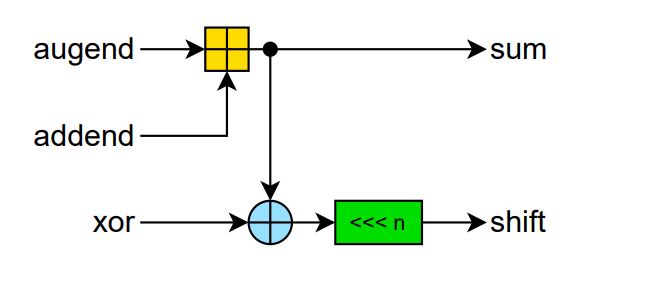
\includegraphics[width=1\linewidth]{arx.png}
  \caption{Bloc ARX}
  \label{fig:arx}
\end{figure}

La valeur de la rotation $r$ dépend de la position du bloc ARX dans la structure QuarterRound
que nous allons ensuite étudier.

\subsection{Simulation et validation}

Les résultats obtenus suite à une simulation sur ModelSim correspondent aux vecteurs de tests
fournis dans le sujet. Cela confirme le bon fonctionnement du module ARX.

\begin{figure}[H]
  \centering
  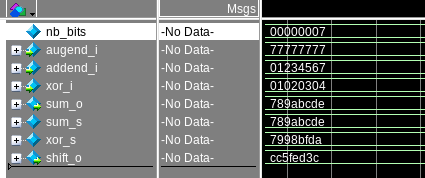
\includegraphics[width=1\linewidth]{arxtb.png}
  \caption{Simulation du module \module{arx} --- vecteurs de test du sujet.}
  \label{fig:sim_arx}
\end{figure}


% ══════════════════════════════════════════════════════════════════════════════
\section{Le QuarterRound}

Le QuarterRound prend en entrée quatre mots de 32~bits (notés $a, b, c, d$) et produit quatre
nouveaux mots en sortie après l'application successive de quatre blocs ARX avec des rotations
différentes (16, 12, 8 et 7~bits). Ce module est, lui aussi, purement \textbf{combinatoire}.

\subsection{Explication théorique}

\begin{align}
  a &\leftarrow a + b;\quad d \leftarrow (d \oplus a) \lll 16 \\
  c &\leftarrow c + d;\quad b \leftarrow (b \oplus c) \lll 12 \\
  a &\leftarrow a + b;\quad d \leftarrow (d \oplus a) \lll 8  \\
  c &\leftarrow c + d;\quad b \leftarrow (b \oplus c) \lll 7
\end{align}

Pour la modélisation, je définis quatre signaux internes afin de relier les blocs ARX.
Le premier, \signal{n1\_s} est la sortie du premier ARX (rotation 16~bits),
\signal{n2\_s} celle du deuxième (rotation 12~bits), \signal{n3\_s} celle du troisième
(rotation 8~bits) et \signal{n4\_s} la sortie finale du quatrième ARX (rotation 7~bits).

Le QuarterRound contient uniquement des blocs combinatoires, en cela, il est un module
purement combinatoire.

\begin{figure}[H]
  \centering
  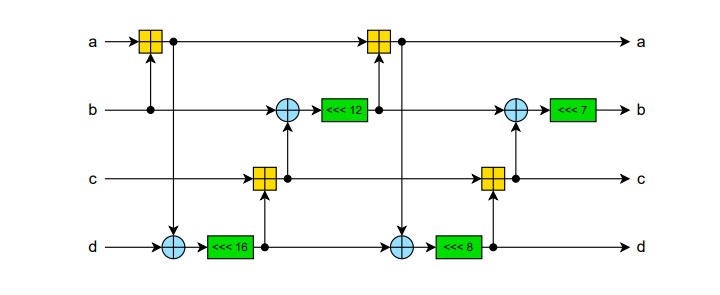
\includegraphics[width=1\linewidth]{quarterround.png}
  \caption{Bloc \module{QuarterRound} .}
  \label{fig:quarterround}
\end{figure}

\subsection{Simulation et validation}


\begin{figure}[H]
  \centering
  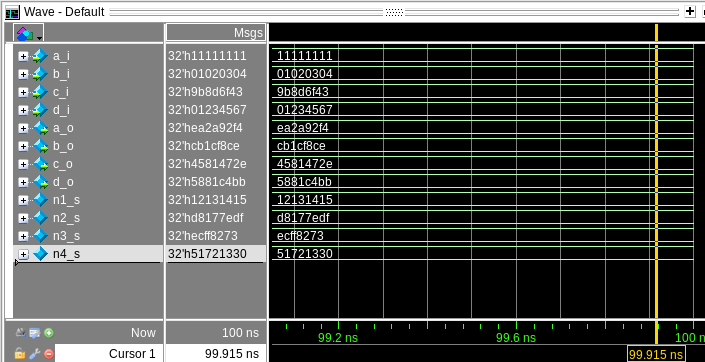
\includegraphics[width=1\linewidth]{quarterroundtb.png}
  \caption{Simulation du module \module{QuarterRound} .}
  \label{fig:quarterround}
\end{figure}


Les résultats obtenus suite à une simulation sur ModelSim correspondent aux vecteurs de tests
fournis dans le sujet. Cela confirme le bon fonctionnement du module QuarterRound.

% ══════════════════════════════════════════════════════════════════════════════
\section{Rondes colonne et rotation de lignes}

L'algorithme ChaCha20 alterne, sur 20~rondes au total, une ronde en colonne et une ronde en
diagonale. Chaque ronde consiste en l'application simultanée de quatre QuarterRounds portant
sur des groupes de quatre mots distincts extraits de la matrice d'état $4\times4$.

\subsection{La ronde en colonne (\texttt{round\_colonne})}

Puisque l'état interne de ChaCha20 est composé de 16 mots de 32~bits, il est nécessaire
d'appliquer quatre fois la fonction QuarterRound.

Les rondes en colonne s'appliquent donc de la façon suivante :

\begin{center}
\begin{tabular}{l}
  $\text{QR}(s_0,\; s_4,\; s_8,\; s_{12})$\\
  $\text{QR}(s_1,\; s_5,\; s_9,\; s_{13})$\\
  $\text{QR}(s_2,\; s_6,\; s_{10},\; s_{14})$\\
  $\text{QR}(s_3,\; s_7,\; s_{11},\; s_{15})$\\
\end{tabular}
\end{center}


\begin{figure}[H]
    \centering
    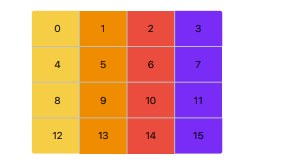
\includegraphics[width=0.4\linewidth]{image.png}
    \caption{Matrice en colonne}
    \label{fig:placeholder}
\end{figure}


\subsection{Simulation des rondes diagonales par rotation de lignes}

Nous venons d'étudier la réalisation des rondes en colonne. Cependant, ChaCha20 est fait de
rondes en colonnes mais aussi de rondes en diagonales.

Les rondes en diagonale s'appliquent de cette façon :

\begin{center}
\begin{tabular}{l}
  $\text{QR}(s_0,\; s_5,\; s_{10},\; s_{15})$\\
  $\text{QR}(s_1,\; s_6,\; s_{11},\; s_{12})$\\
  $\text{QR}(s_2,\; s_7,\; s_8,\; s_{13})$\\
  $\text{QR}(s_3,\; s_4,\; s_9,\; s_{14})$\\
\end{tabular}
\end{center}


\begin{figure}[H]
    \centering
    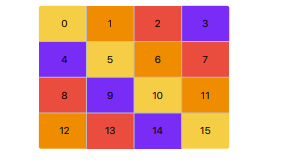
\includegraphics[width=0.4\linewidth]{diago.png}
    \caption{Matrice en diagonale}
    \label{fig:placeholder}
\end{figure}

Plutôt que de créer un module de ronde diagonale dédié, je réalise la ronde diagonale en
réutilisant \module{round\_colonne}, précédé d'une permutation des lignes par le module
\module{rotation}.

Le module \module{rotation} fonctionne à l'aide d'une variable de type \signal{rotation\_t}
définie dans le package \module{rotation\_pck.sv}. Ce type contient deux valeurs de type
logique \signal{COL2DIAG} et \signal{DIAG2COL} qui indiquent de quelle façon transformer la
matrice en vue de la prochaine ronde.

Afin de tester le fonctionnement de ma fonction rotation, j'initialise l'état d'entrée avec
des valeurs distinctes selon leur colonne (0, 1, 2, 3). Je leur applique d'abord la
transformation \signal{COL2DIAG} pour commencer et je vérifie que les cases sont bien décalées,
puis j'applique ensuite la transformation \signal{DIAG2COL} sur le résultat obtenu. Les deux
transformations étant inverses, on retrouve bien l'état initial.
($\text{COL2DIAG} \times \text{DIAG2COL} = \text{identité}$)

\begin{figure}
    \centering
    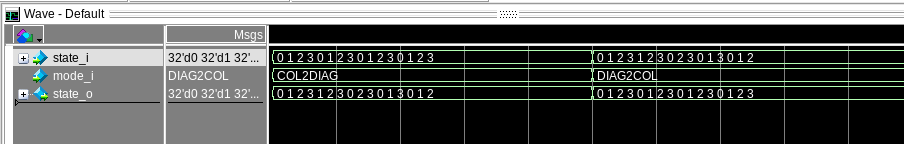
\includegraphics[width=1\linewidth]{rotationtb.png}
    \caption{Simulation du module \module{rotation}}
    \label{fig:placeholder}
\end{figure}


\textbf{Note~:} afin d'afficher tous les bits des signaux \signal{state\_i} et \signal{state\_o}
sur l'écran wave, j'ai changé leur mode d'affichage en base décimale.


\subsubsection{Multiplexeur d'initialisation}

Dans le module \module{chacha\_bloc}, un multiplexeur sélectionne l'état qui sera traité par le bloc \module{round\_colonne}. Lors du premier cycle (\signal{init\_i} = 1), le multiplexeur sélectionne l'état initial \signal{init\_state\_i} afin de l'injecter dans la première ronde. Pour les cycles suivants (\signal{init\_i} = 0), il sélectionne la sortie qui représente le résultat de la ronde précédente.

\subsubsection{Simulation et validation}

Les résultats obtenus suite à une simulation correspondent aux vecteurs de tests fournis. Le testbench commence par initialiser le \signal{keystream\_i} à zéro, puis donne une assigne des valeurs reconnaissable  afin de les identifier sur modelsim. Le compteur est ensuite incrémenté et je remarque que les 

Le testbench initialise le \signal{keystream\_i} à zéro, puis force \signal{keystream\_i[0]} = \texttt{0x00000001} et \signal{keystream\_i[4]} = \texttt{0x00000002} afin d'identifier facilement quel quart est sélectionné. Le compteur \signal{cpt\_i} est ensuite balayé sur ses quatre valeurs possibles avec un délai de 50~ns entre chaque changement. Cela confirme le bon fonctionnement du module.

\begin{figure}[H]
  \centering
  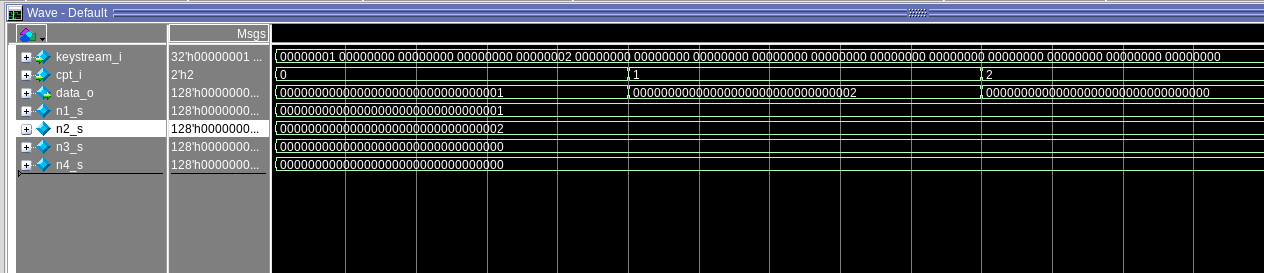
\includegraphics[width=\linewidth]{muxtb.png}
  \caption{Simulation du multiplexeur d'initialisation dans \module{chacha\_bloc}.}
  \label{fig:sim_mux}
\end{figure}
% ══════════════════════════════════════════════════════════════════════════════
\section{Bloc ChaCha20 (\texttt{chacha\_bloc})}

Ce module utilise les fonctions définies précédemment afin de réaliser 20~rondes de
transformation (10 en colonnes et 10 en diagonales) avec un état interne de 512~bits.

Un signal \signal{init\_i} permet de charger l'état initial et  \signal{reg\_sel\_i} sélectionne si l'on fourni au registre le résultat de la ronde ou
 l'état initial. Après les 20~rondes, le keystream est généré à partir d'une addition  (modulo $2^{32}$) entre l'état final et l'état initial.

Le module \module{chacha\_bloc} intègre un registre d'état (\module{registre\_d}) qui mémorise
le résultat de chaque ronde et le fournit en entrée de la ronde suivante. Ce mécanisme rend le
module \textbf{séquentiel}.

\subsection{Architecture interne}

Le bloc ChaCha20 importe les modules définis précédemment (\module{round\_colonne},
\module{registre\_d}, \module{rotation}, \module{additionneur}) afin de réaliser 20~rondes dont
10 en colonnes et 10 en diagonales. Suite à cela, l'additionneur réalise une addition modulo
$2^{32}$ entre la sortie des 20~rondes et l'état initial.

Durant l'exécution du ChaChabloc, un multiplexeur en entrée sélectionne l'état initial pour le
charger dans la première ronde ou l'état du registre pour le calcul des rondes suivantes.

À l'intérieur des rondes, le bloc \module{round\_colonne} applique quatre QuarterRounds,
\module{rotation} permute les cases de la matrice, puis Reg State mémorise l'état courant.

\begin{figure}[H]
\centering
\scalebox{0.75}{%
\begin{circuitikz}
\tikzstyle{every node}=[font=\fontsize{18.2pt}{23.7pt}\selectfont]
\draw (4.875,14) -- (5.375,14);
\draw (4.875,14.5) -- (5.375,14.5);
\draw  (5.375,13.5) -- (5.375,15) -- (6.25,14.5) -- (6.25, 14) -- (5.375,13.5);
\draw (6.25,14.25) -- (6.75,14.25);
\draw (5.875,13) -- (5.875,13.785714285714285);
\node [font=\fontsize{18.2pt}{23.7pt}\selectfont] at (5.875,14.25) {};
\draw  (7.25,15.5) rectangle (9,13);
\draw  (10.375,15.5) rectangle (12.125,13);
\draw [short] (6.25,14.25) -- (7.25,14.25);
\draw [-{Stealth[scale=1.5]}] (9,14.25) -- (10.375,14.25);
\draw [-{Stealth[scale=1.5]}] (12.125,14.25) -- (13.75,14.25);
\draw  (13.75,15.5) rectangle (15.5,13);
\node [font=\fontsize{6.3pt}{8.1pt}\selectfont, inner xsep=0.080cm, inner ysep=0.085cm, rounded corners=0.000cm] at (5.5,14) {1};
\node [font=\fontsize{6.3pt}{8.1pt}\selectfont, inner xsep=0.080cm, inner ysep=0.085cm, rounded corners=0.000cm] at (5.5,14.5) {0};
\node [font=\fontsize{5.1pt}{6.7pt}\selectfont, inner xsep=0.080cm, inner ysep=0.085cm, rounded corners=0.000cm] at (4.375,14) {$init\_state\_i$};
\node [font=\fontsize{5.1pt}{6.7pt}\selectfont, inner xsep=0.080cm, inner ysep=0.085cm, rounded corners=0.000cm] at (9.625,14.625) {$state\_t$};
\draw (9.375,14) -- (9.75,14.375);
\draw (12.875,14.375) -- (12.5,14);
\node [font=\fontsize{5.1pt}{6.7pt}\selectfont, inner xsep=0.080cm, inner ysep=0.085cm, rounded corners=0.000cm] at (12.875,14.625) {$state\_t$};
\draw (15.5,15.25) -- (16,15.25);
\draw (14.625,15.5) -- (14.625,16);
\draw (14.625,13) -- (14.625,12.5);
\node [font=\fontsize{5.1pt}{6.7pt}\selectfont, inner xsep=0.080cm, inner ysep=0.085cm, rounded corners=0.000cm] at (16.375,15.25) {$state\_o$};
\node [font=\fontsize{5.1pt}{6.7pt}\selectfont, inner xsep=0.080cm, inner ysep=0.085cm, rounded corners=0.000cm] at (14.625,16.25) {$resetb\_i$};
\draw  (13.375,10.375) rectangle (16.625,8.75);
\node [font=\fontsize{10.2pt}{13.3pt}\selectfont, inner xsep=0.080cm, inner ysep=0.085cm, rounded corners=0.020cm] at (15.125,9.5) {$Addition\ 2^{32}$};
\node [font=\fontsize{10.2pt}{13.3pt}\selectfont, inner xsep=0.080cm, inner ysep=0.085cm, rounded corners=0.020cm] at (8.125,14.25) {$Round$};
\node [font=\fontsize{9.1pt}{11.8pt}\selectfont, inner xsep=0.080cm, inner ysep=0.085cm, rounded corners=0.020cm] at (11.25,14.25) {$COL/DIAG$};
\node [font=\fontsize{9.1pt}{11.8pt}\selectfont, inner xsep=0.080cm, inner ysep=0.085cm, rounded corners=0.020cm] at (14.625,14.5) {$Reg\ State$};
\draw [short] (4.875,14.5) -- (4.875,17);
\draw [short] (4.875,17) -- (16,17);
\draw [short] (16,17) -- (16,15.25);
\draw [short] (16,15.25) -- (16,10.375);
\draw [short] (4.875,14) -- (4.875,9.875);
\draw [short] (4.875,9.875) -- (13.375,9.75);
\draw (9.875,10) -- (9.5,9.625);
\draw (16.25,11.5) -- (15.875,11.125);
\node [font=\fontsize{5.1pt}{6.7pt}\selectfont, inner xsep=0.080cm, inner ysep=0.085cm, rounded corners=0.000cm] at (16.25,10.625) {$a\_i$};
\node [font=\fontsize{5.1pt}{6.7pt}\selectfont, inner xsep=0.080cm, inner ysep=0.085cm, rounded corners=0.000cm] at (13.125,10) {$b\_i$};
\draw [-{Stealth[scale=1.5]}] (12.75,9.75) -- (13.375,9.75);
\draw [-{Stealth[scale=1.5]}] (16,11) -- (16,10.375);
\draw [short] (15.125,8.75) -- (15.125,8.25);
\node [font=\fontsize{5.1pt}{6.7pt}\selectfont, inner xsep=0.080cm, inner ysep=0.085cm, rounded corners=0.000cm] at (15.125,8.125) {$Keystream\_o$};
\node [font=\fontsize{5.1pt}{6.7pt}\selectfont, inner xsep=0.080cm, inner ysep=0.085cm, rounded corners=0.000cm] at (9.625,10.125) {$512$};
\node [font=\fontsize{5.1pt}{6.7pt}\selectfont, inner xsep=0.080cm, inner ysep=0.085cm, rounded corners=0.000cm] at (16.375,11.25) {$512$};
\node [font=\fontsize{5.1pt}{6.7pt}\selectfont, inner xsep=0.080cm, inner ysep=0.085cm, rounded corners=0.000cm] at (4.375,14.625) {$state\_s$};
\node [font=\fontsize{5.1pt}{6.7pt}\selectfont, inner xsep=0.080cm, inner ysep=0.085cm, rounded corners=0.000cm] at (14.625,12.25) {$Clock\_i$};
\node [font=\fontsize{5.1pt}{6.7pt}\selectfont, inner xsep=0.080cm, inner ysep=0.085cm, rounded corners=0.000cm] at (5.875,12.875) {$Select\_i$};
\end{circuitikz}
}%
\caption{Architecture interne du module \module{chacha\_bloc}.}
\label{fig:chacha_bloc}
\end{figure}

\subsection{Interface du module}

\begin{lstlisting}[caption={Interface du module \texttt{chacha\_bloc}}]
module chacha_bloc
import chacha_pck::*;
import rotation_pck::*;
(
  input  logic      clock_i,
  input  logic      resetb_i,
  input  state_t    init_state_i, // etat initial S_init
  input  logic      init_i,       // 1 = premier cycle (injecter S_init)
  input  rotation_t rotation_i,   // COL2DIAG ou DIAG2COL
  input  logic      reg_sel_i,    // enable registre d'etat
  output state_t    keystream_o   // keystream apres addition (512 bits)
);
\end{lstlisting}

\subsection{Simulation et validation}

Afin de tester le bon fonctionnement du bloc ChaCha20, je réalise un testbench dans lequel
j'initialise l'entrée à partir de celle fournie à la fin du sujet. Je réalise 20~rondes en
alternant les rondes en colonne et en diagonale puis je constate le fait que la valeur obtenue
en sortie correspond à la valeur attendue à la fin du sujet.

Je ne suis pas parvenu à obtenir la même valeur et n'ai malheureusement pas eu le temps de
proprement déboguer.


\begin{figure}
    \centering
    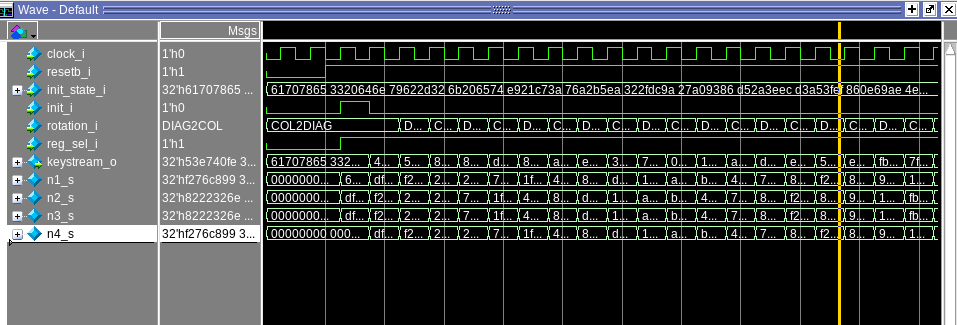
\includegraphics[width=1\linewidth]{bloctb.png}
      \caption{Simulation du module \module{chacha\_bloc}.}
    \label{fig:sim_chacha_bloc}
\end{figure}


% ══════════════════════════════════════════════════════════════════════════════
\section{Machine d'états finis (FSM)}

La machine d'états finis (FSM) séquence les opérations du chiffrement en générant les signaux
de contrôle à destination des autres modules (\module{chacha\_bloc}, compteur, registre de
sortie, module XOR).

\subsection{Présentation générale}

\begin{tcolorbox}[defbox, title={Type de machine}]
Il s'agit d'une machine de Moore, c'est-à-dire que les sorties ne dépendent uniquement de
l'état courant. Cependant, trois sorties --- \signal{init\_o}, \signal{rotation\_o} et
\signal{xor\_cpt\_o} --- dépendent également du signal \signal{cpt\_i} en plus de l'état
courant, introduisant un comportement de Mealy partiel pour ces signaux.
\end{tcolorbox}


\subsection{Graphe des états}

\begin{figure}[H]
\centering
\scalebox{0.45}{%
\begin{circuitikz}
\tikzstyle{every node}=[font=\fontsize{18.2pt}{23.7pt}\selectfont]

% ── IDLE ──────────────────────────────────────────────────────────────────
\draw (7.5,28) ellipse (2.125cm and 1.125cm)
  node[inner xsep=0.08cm, inner ysep=0.085cm, rounded corners=0.02cm]
  {\fontsize{18.2pt}{23.7pt}\selectfont Idle};

\draw [-{Stealth[scale=1.5]}]
  (9.5,28.25) .. controls (11.25,28.5) and (11,27.875) .. (9.625,27.625);
\node [font=\fontsize{8.0pt}{10.4pt}\selectfont]
  at (12.25,28.125) {$start\_i == 1'b0$};

\draw [-{Stealth[scale=1.5]}] (7.5,26.875) -- (7.5,24.125);
\node [font=\fontsize{8.0pt}{10.4pt}\selectfont]
  at (9.75,25.5) {$start\_i == 1'b1$};

% ── INIT_CPT ──────────────────────────────────────────────────────────────
\draw (7.5,23) ellipse (2.125cm and 1.125cm)
  node[inner xsep=0.08cm, inner ysep=0.085cm, rounded corners=0.02cm]
  {\fontsize{18.2pt}{23.7pt}\selectfont $init\_cpt$};

\node [font=\fontsize{8.0pt}{10.4pt}\selectfont, anchor=west,
       color={rgb,255:red,255;green,0;blue,0}]
  at (15.5,23.4) {$init\_cpt\_o = 1$};
\node [font=\fontsize{8.0pt}{10.4pt}\selectfont, anchor=west,
       color={rgb,255:red,255;green,0;blue,0}]
  at (15.5,23.0) {$en\_cpt\_o = 1$};

\draw [-{Stealth[scale=1.5]}] (7.5,21.875) -- (7.5,19.125);

% ── CHACHA_BLOC ───────────────────────────────────────────────────────────
\draw (7.5,18) ellipse (2.125cm and 1.125cm)
  node[inner xsep=0.08cm, inner ysep=0.085cm, rounded corners=0.02cm]
  {\fontsize{18.2pt}{23.7pt}\selectfont $chacha\_bloc$};

\draw [-{Stealth[scale=1.5]}]
  (9.5,18.25) .. controls (11.25,18.5) and (11,17.875) .. (9.625,17.625);
\node [font=\fontsize{8.0pt}{10.4pt}\selectfont]
  at (12.25,18.125) {$cpt\_i < 19$};

\node [font=\fontsize{8.0pt}{10.4pt}\selectfont, anchor=west,
       color={rgb,255:red,255;green,0;blue,0}]
  at (15.5,19.5) {$en\_cpt\_o = 1$};
\node [font=\fontsize{8.0pt}{10.4pt}\selectfont, anchor=west,
       color={rgb,255:red,255;green,0;blue,0}]
  at (15.5,19.1) {$reg\_sel\_o = 1$};
\node [font=\fontsize{8.0pt}{10.4pt}\selectfont, anchor=west,
       color={rgb,255:red,255;green,0;blue,0}]
  at (15.5,18.65) {si $cpt\_i == 0$ :};
\node [font=\fontsize{8.0pt}{10.4pt}\selectfont, anchor=west,
       color={rgb,255:red,255;green,0;blue,0}]
  at (16.3,18.25) {$init\_o = 1$};
\node [font=\fontsize{8.0pt}{10.4pt}\selectfont, anchor=west,
       color={rgb,255:red,255;green,0;blue,0}]
  at (15.5,17.85) {sinon :};
\node [font=\fontsize{8.0pt}{10.4pt}\selectfont, anchor=west,
       color={rgb,255:red,255;green,0;blue,0}]
  at (16.3,17.45) {$init\_o = 0$};
\node [font=\fontsize{8.0pt}{10.4pt}\selectfont, anchor=west,
       color={rgb,255:red,255;green,0;blue,0}]
  at (15.5,17.0) {si $cpt\_lsb$ :};
\node [font=\fontsize{8.0pt}{10.4pt}\selectfont, anchor=west,
       color={rgb,255:red,255;green,0;blue,0}]
  at (16.3,16.6) {$rotation\_o = $ DIAG2COL};
\node [font=\fontsize{8.0pt}{10.4pt}\selectfont, anchor=west,
       color={rgb,255:red,255;green,0;blue,0}]
  at (15.5,16.2) {sinon :};
\node [font=\fontsize{8.0pt}{10.4pt}\selectfont, anchor=west,
       color={rgb,255:red,255;green,0;blue,0}]
  at (16.3,15.8) {$rotation\_o = $ COL2DIAG};

\draw [-{Stealth[scale=1.5]}] (7.5,16.875) -- (7.5,14.125);
\node [font=\fontsize{8.0pt}{10.4pt}\selectfont]
  at (9.5,15.5) {$cpt\_i \geq 19$};

% ── ADDITION ──────────────────────────────────────────────────────────────
\draw (7.5,13) ellipse (2.125cm and 1.125cm)
  node[inner xsep=0.08cm, inner ysep=0.085cm, rounded corners=0.02cm]
  {\fontsize{18.2pt}{23.7pt}\selectfont $addition$};

\node [font=\fontsize{8.0pt}{10.4pt}\selectfont, anchor=west,
       color={rgb,255:red,255;green,0;blue,0}]
  at (15.5,13.5) {$keystream\_sel\_o = 1$};
\node [font=\fontsize{8.0pt}{10.4pt}\selectfont, anchor=west,
       color={rgb,255:red,255;green,0;blue,0}]
  at (15.5,13.1) {$init\_cpt\_o = 1$};
\node [font=\fontsize{8.0pt}{10.4pt}\selectfont, anchor=west,
       color={rgb,255:red,255;green,0;blue,0}]
  at (15.5,12.7) {$en\_cpt\_o = 1$};

\draw [-{Stealth[scale=1.5]}] (7.5,11.875) -- (7.5,9.125);

% ── INIT_LOOP ─────────────────────────────────────────────────────────────
\draw (7.5,8) ellipse (2.125cm and 1.125cm)
  node[inner xsep=0.08cm, inner ysep=0.085cm, rounded corners=0.02cm]
  {\fontsize{18.2pt}{23.7pt}\selectfont $init\_loop$};

\draw [-{Stealth[scale=1.5]}]
  (9.5,8.25) .. controls (11.25,8.5) and (11,7.875) .. (9.625,7.625);
\node [font=\fontsize{8.0pt}{10.4pt}\selectfont]
  at (12.75,8.125) {$data\_valid\_i == 1'b0$};

\node [font=\fontsize{8.0pt}{10.4pt}\selectfont, anchor=west,
       color={rgb,255:red,255;green,0;blue,0}]
  at (15.5,8.1) {$end\_o = 1$};

\draw [-{Stealth[scale=1.5]}] (7.5,6.875) -- (7.5,4.125);
\node [font=\fontsize{8.0pt}{10.4pt}\selectfont]
  at (9.75,5.5) {$data\_valid\_i == 1'b1$};

% ── XOR_STATE ─────────────────────────────────────────────────────────────
\draw (7.5,3) ellipse (2.125cm and 1.125cm)
  node[inner xsep=0.08cm, inner ysep=0.085cm, rounded corners=0.02cm]
  {\fontsize{18.2pt}{23.7pt}\selectfont $xor\_state$};

\node [font=\fontsize{8.0pt}{10.4pt}\selectfont, anchor=west,
       color={rgb,255:red,255;green,0;blue,0}]
  at (15.5,3.5) {$cipher\_reg\_sel\_o = 1$};
\node [font=\fontsize{8.0pt}{10.4pt}\selectfont, anchor=west,
       color={rgb,255:red,255;green,0;blue,0}]
  at (15.5,3.1) {$en\_cpt\_o = 1$};
\node [font=\fontsize{8.0pt}{10.4pt}\selectfont, anchor=west,
       color={rgb,255:red,255;green,0;blue,0}]
  at (15.5,2.7) {$xor\_cpt\_o = cpt\_i[1:0]$};

\draw [-{Stealth[scale=1.5]}] (7.5,1.875) -- (7.5,-0.875);

% ── END_LOOP ──────────────────────────────────────────────────────────────
\draw (7.5,-2) ellipse (2.125cm and 1.125cm)
  node[inner xsep=0.08cm, inner ysep=0.085cm, rounded corners=0.02cm]
  {\fontsize{18.2pt}{23.7pt}\selectfont $end\_loop$};

\node [font=\fontsize{8.0pt}{10.4pt}\selectfont, anchor=west,
       color={rgb,255:red,255;green,0;blue,0}]
  at (15.5,-1.9) {$cipher\_valid\_o = 1$};

\draw [-{Stealth[scale=1.5]}]
  (5.375,-2) .. controls (2,-2) and (2,8) .. (5.375,8);
\node [font=\fontsize{8.0pt}{10.4pt}\selectfont]
  at (2.5,3) {$cpt\_i < 3$};

\draw [-{Stealth[scale=1.5]}] (7.5,-3.125) -- (7.5,-5.875);
\node [font=\fontsize{8.0pt}{10.4pt}\selectfont]
  at (9.5,-4.5) {$cpt\_i \geq 3$};

% ── FIN ───────────────────────────────────────────────────────────────────
\draw (7.5,-7) ellipse (2.125cm and 1.125cm)
  node[inner xsep=0.08cm, inner ysep=0.085cm, rounded corners=0.02cm]
  {\fontsize{18.2pt}{23.7pt}\selectfont $fin$};

\node [font=\fontsize{8.0pt}{10.4pt}\selectfont, anchor=west,
       color={rgb,255:red,255;green,0;blue,0}]
  at (15.5,-7.0) {$init\_cpt\_o = 1$};

\draw [-{Stealth[scale=1.5]}]
  (5.375,-7) .. controls (-1,-7) and (-1,28) .. (5.375,28);

\end{circuitikz}
}%
\caption{Graphe des états de la FSM \module{chacha20\_top}.}
\label{fig:fsm}
\end{figure}

\subsection{Table des sorties}

\begin{center}
\small\setlength{\tabcolsep}{4pt}
\begin{tabular}{lcccccccc}
  \toprule
  \textbf{Signal}
    & \etat{idle} & \etat{init\_cpt} & \etat{chacha} & \etat{addition}
    & \etat{init\_loop} & \etat{xor} & \etat{end\_loop} & \etat{fin} \\
  \midrule
  \signal{en\_cpt\_o}           & 0 & 1 & 1 & 1 & 0 & 1 & 0 & 0 \\
  \signal{init\_cpt\_o}         & 0 & 1 & 0 & 1 & 0 & 0 & 0 & 1 \\
  \signal{init\_o}              & 0 & 0 & $\star$ & 0 & 0 & 0 & 0 & 0 \\
  \signal{reg\_sel\_o}          & 0 & 0 & 1 & 0 & 0 & 0 & 0 & 0 \\
  \signal{keystream\_sel\_o}    & 0 & 0 & 0 & 1 & 0 & 0 & 0 & 0 \\
  \signal{cipher\_reg\_sel\_o}  & 0 & 0 & 0 & 0 & 0 & 1 & 0 & 0 \\
  \signal{cipher\_valid\_o}     & 0 & 0 & 0 & 0 & 0 & 0 & 1 & 0 \\
  \signal{end\_o}               & 0 & 0 & 0 & 0 & 1 & 0 & 0 & 0 \\
  \bottomrule
\end{tabular}
\end{center}
\noindent$\star$ : \signal{init\_o=1} uniquement lorsque \signal{cpt\_i=0}.

\subsection{Simulation et validation}

Un testbench instancie la FSM et le compteur. Le signal \signal{start\_i} est activé afin de
vérifier le bon fonctionnement de la FSM, puis le signal reset est activé et relâché afin que
la FSM commence dans son premier état.

\begin{figure}
    \centering
    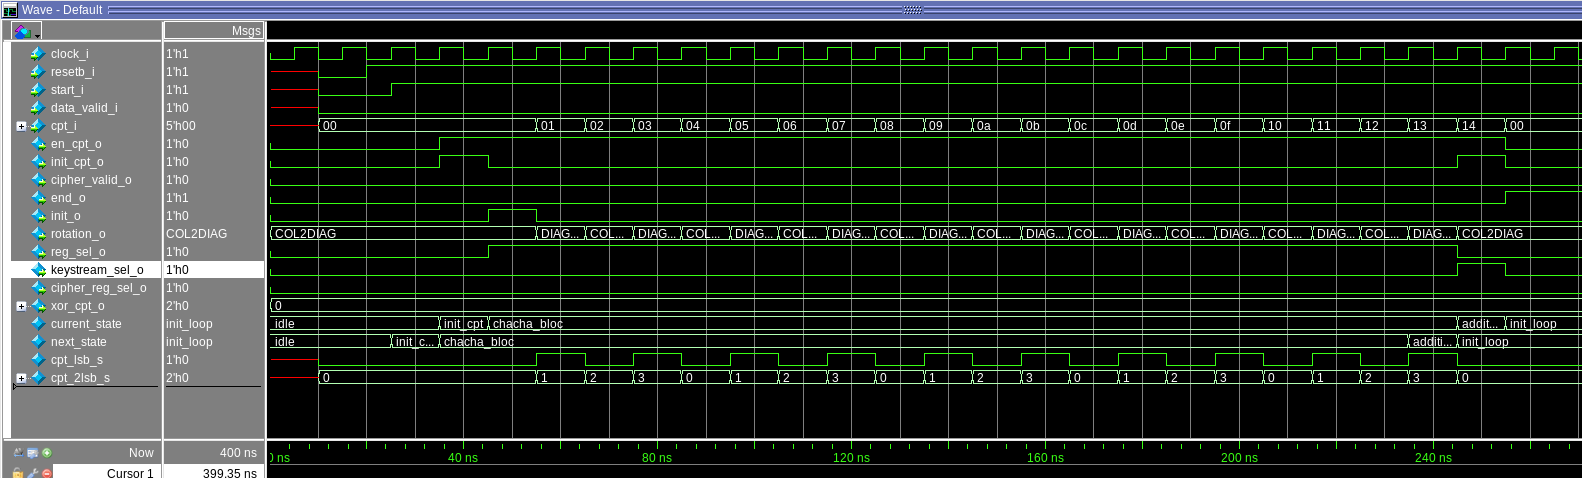
\includegraphics[width=1\linewidth]{tbfsm.png}
    \caption{Simulation de la FSM --- enchaînement des états et signaux de contrôle.}
    \label{fig:sim_fsm}
\end{figure}



% ══════════════════════════════════════════════════════════════════════════════
\section{Module top-level (\texttt{chacha20\_top})}

Le module \module{chacha20\_top} est le plus haut niveau d'intégration. Il instancie et
interconnecte l'ensemble des modules développés au long du projet dans l'objectif de former
le circuit.

Concrètement, ce module construit l'état initial à partir de la constante, de la clé et du
nonce, le fournit au bloc \module{chacha\_bloc}, puis récupère le keystream produit après les
20~rondes. Il intègre également le compteur de rondes qui indique à la machine d'état le numéro
de la ronde courante, le module XOR qui chiffre chaque bloc de 16~octets du message en
appliquant un XOR avec la tranche correspondante du keystream, et un registre de 512~bits qui
mémorise le keystream.

\subsection{Architecture globale}

\begin{figure}[H]
\centering
\resizebox{\linewidth}{!}{%
\begin{tikzpicture}[
  font=\scriptsize,
  fleche/.style={-{Stealth[scale=1.5]}},
  txt/.style={font=\fontsize{7pt}{9pt}\selectfont}
]
% ── Blocs ─────────────────────────────────────────────────────────────────
\draw[fill=lightblue, draw=maincolor, rounded corners=2pt]
  (3,17.5) rectangle (6,13);
\node[font=\normalsize\bfseries\color{maincolor}] at (4.5,15.25) {FSM};

\draw[fill=lightblue, draw=maincolor, rounded corners=2pt]
  (3,11.5) rectangle (6,9.5);
\node[font=\small\color{maincolor}] at (4.5,10.5) {compteur\_init};

\draw[fill=lightblue, draw=maincolor, rounded corners=2pt]
  (8,17.5) rectangle (12,13);
\node[font=\normalsize\bfseries\color{maincolor}] at (10,15.25) {chacha\_bloc};

\draw[fill=lightblue, draw=maincolor, rounded corners=2pt]
  (14,17.5) rectangle (17.5,13);
\node[font=\normalsize\bfseries\color{maincolor}] at (15.75,15.25) {reg512};

\draw[fill=lightblue, draw=maincolor, rounded corners=2pt]
  (19.5,17.5) rectangle (23,13);
\node[font=\normalsize\bfseries\color{maincolor}] at (21.25,15.25) {xor\_module};

\draw[fill=lightblue, draw=maincolor, rounded corners=2pt]
  (25,17.5) rectangle (28.5,13);
\node[font=\small\bfseries\color{maincolor}, align=center] at (26.75,15.25)
  {always\_ff\\cipher\_o};

% ── FSM -> chacha_bloc ────────────────────────────────────────────────────
\draw [-{Stealth[scale=1.5]}] (6,16.5) -- (8,16.5) node[midway, above, txt] {init\_o};
\draw [-{Stealth[scale=1.5]}] (6,15.25) -- (8,15.25) node[midway, above, txt] {rotation\_o};
\draw [-{Stealth[scale=1.5]}] (6,14) -- (8,14) node[midway, above, txt] {reg\_sel\_o};

% ── FSM -> contrôles supérieurs ───────────────────────────────────────────
\draw [-{Stealth[scale=1.5]}] (4.5,17.5) .. controls (4.5,19.5) and (15.75,19.5) .. (15.75,17.5);
\node [txt] at (10.125,19.7) {keystream\_sel\_o};

\draw [-{Stealth[scale=1.5]}] (4.1,17.5) .. controls (4.1,20.5) and (21.25,20.5) .. (21.25,17.5);
\node [txt] at (12.6,20.7) {xor\_cpt\_o[1:0]};

\draw [-{Stealth[scale=1.5]}] (3.7,17.5) .. controls (3.7,21.5) and (26.75,21.5) .. (26.75,17.5);
\node [txt] at (15.2,21.7) {cipher\_reg\_sel\_o};

% ── FSM <-> compteur ──────────────────────────────────────────────────────
\draw [-{Stealth[scale=1.5]}] (3.5,13) -- (3.5,11.5) node[midway, left, txt] {en\_cpt};
\draw [-{Stealth[scale=1.5]}] (4.5,13) -- (4.5,11.5) node[midway, right, txt] {init\_cpt};
\draw [-{Stealth[scale=1.5]}] (5.5,11.5) .. controls (5.5,8.0) and (7.0,8.0) .. (7.0,11.0)
  -- (7.0,13.5) -- (6,13.5);
\node [txt] at (6.25,7.8) {cpt\_i[4:0]};

% ── Flux de données ───────────────────────────────────────────────────────
\draw [-{Stealth[scale=1.5]}] (12,15.25) -- (14,15.25) node[midway, above, txt] {keystream\_s};
\draw [-{Stealth[scale=1.5]}] (17.5,15.25) -- (19.5,15.25) node[midway, above, txt] {ks\_slice[127:0]};
\draw [-{Stealth[scale=1.5]}] (23,15.25) -- (25,15.25) node[midway, above, txt] {cipher\_comb};

% ── Feedback reg512 -> chacha_bloc ────────────────────────────────────────
\draw [-{Stealth[scale=1.5]}] (15.75,13) .. controls (15.75,9.5) and (10,9.5) .. (10,13);
\node [txt] at (12.875,9.3) {feedback n4\_s};

% ── Entrées externes ──────────────────────────────────────────────────────
\draw [-{Stealth[scale=1.5]}] (1,16.8) -- (3,16.8) node[at start, left, txt] {start\_i};
\draw [-{Stealth[scale=1.5]}] (1,15.8) -- (3,15.8) node[at start, left, txt] {data\_valid\_i};
\draw [-{Stealth[scale=1.5]}] (1,14.8) -- (3,14.8) node[at start, left, txt] {clock\_i};
\draw [-{Stealth[scale=1.5]}] (1,13.8) -- (3,13.8) node[at start, left, txt] {resetb\_i};
\draw [-{Stealth[scale=1.5]}] (6.5,14.5) -- (8,14.5) node[at start, left, txt] {key\_i};
\draw [-{Stealth[scale=1.5]}] (6.5,13.5) -- (8,13.5) node[at start, left, txt] {nonce\_i};
\draw [-{Stealth[scale=1.5]}] (18,14.25) -- (19.5,14.25) node[at start, left, txt] {data\_i};

% ── Sorties ───────────────────────────────────────────────────────────────
\draw [-{Stealth[scale=1.5]}] (28.5,15.25) -- (30.5,15.25) node[at end, right, txt] {cipher\_o};
\draw [-{Stealth[scale=1.5]}] (4.5,17.5) -- (4.5,22.5) -- (30.5,22.5)
  node[at end, right, txt] {cipher\_valid\_o};
\draw [-{Stealth[scale=1.5]}] (4.8,17.5) -- (4.8,23.2) -- (30.5,23.2)
  node[at end, right, txt] {end\_o};
\end{tikzpicture}%
}% end resizebox
\caption{Architecture globale du module \module{chacha20\_top}.}
\label{fig:top}
\end{figure}

\subsection{Interface du module}

\begin{lstlisting}[caption={Interface du module \texttt{chacha20\_top}}]
module chacha20_top
import chacha_pck::*;
import rotation_pck::*;
(
  input  logic         clock_i,
  input  logic         resetb_i,
  input  logic         start_i,        // demarre le chiffrement
  input  logic [127:0] data_i,         // texte clair (128 bits)
  input  logic         data_valid_i,   // donnee disponible
  input  logic [255:0] key_i,          // cle secrete (256 bits)
  input  logic [95:0]  nonce_i,        // nonce (96 bits)
  output logic [127:0] cipher_o,       // texte chiffre (128 bits)
  output logic         cipher_valid_o, // bloc chiffre disponible
  output logic         end_o           // FSM prete a recevoir du texte
);
\end{lstlisting}

\subsection{Compteur de rondes (\texttt{compteur\_init})}

Le module fonctionne de la manière suivante : lorsque \signal{resetb\_i=0}, le compteur est
réinitialisé à~0. Lorsque \signal{resetb\_i=1} et que le write enable \signal{en\_i} est actif,
si \signal{init\_i=1}, le compteur est remis à~0. Sinon, le compteur s'incrémente de~1 à chaque
front montant d'horloge.

Le compteur renvoie une valeur sur 5~bits, ce qui permet de compter jusqu'à~31. Cela est
suffisant pour les deux usages : les 20~rondes ChaCha (valeurs jusque~19) et les blocs XOR.

Ce module étant fourni et déjà validé, aucun testbench dédié n'a été réalisé.

\subsection{Module XOR (\texttt{xor\_module})}

Le module \module{xor\_module} effectue un ou-exclusif bit à bit sur 128~bits entre une tranche
du keystream et le bloc de texte clair \signal{data\_i}, produisant le bloc chiffré
\signal{cipher\_o}.

Afin de tester notre module XOR, il suffit de rentrer deux mots en entrée et de vérifier que la
sortie correspond bien à l'application bit-à-bit d'un ou-exclusif.

\begin{figure}
    \centering
    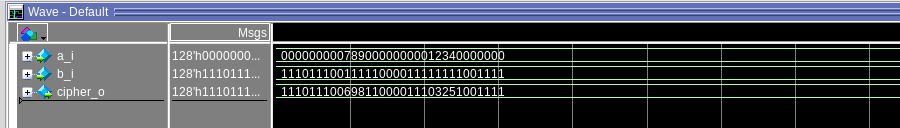
\includegraphics[width=1\linewidth]{xormtb.png}
    \caption{Simulation du module XOR }
    \label{fig:placeholder}
\end{figure}

\subsection{Registre de keystream (\texttt{reg512})}

Ce registre est utile à la mémorisation du keystream suite à l'exécution des 20~rondes. Ainsi,
on manipule des données de type \signal{state\_t}, la matrice de 16 cases de 32~bits.

Tout comme pour le module compteur, on se sert d'un reset actif bas. Lorsque le reset est
inactif, à chaque front montant d'horloge et uniquement si \signal{sel\_i=1}, la sortie
\signal{state\_o} prend la valeur de l'entrée \signal{state\_i}.

\subsection{Intégration et validation}

Je construis l'état initial à partir des vecteurs de tests fournies dans l'énoncé.

Durant l'exécution, la machine d'état permet l'alternance des rondes en colonnes et en
diagonales à partir du signal interne \signal{rotation\_s}. Je vérifie sur le chronogramme que
ce signal bascule parfaitement entre \signal{COL2DIAG} et \signal{DIAG2COL} à chaque cycle,
enchaînant ainsi les 10~cycles complets (soit les 20~rondes cumulées suivies par le compteur
\signal{cpt\_s}). La bonne exécution du chemin de données est validée à la fin du calcul
lorsque le signal \signal{end\_o} passe à~1 et que le résultat final obtenu sur la sortie
\signal{cipher\_o} concorde parfaitement avec la valeur de chiffrement théorique attendue.

Je vérifie la présence du signal \signal{cipher\_valid\_o} délivré par ma machine d'état.

\begin{figure}[H] % Force la position ici
    \centering
    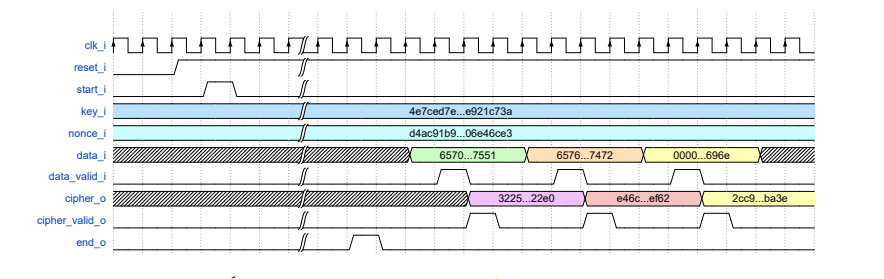
\includegraphics[width=1\linewidth]{bloc.png}
    \caption{Fonctionnement interne de l'algorithme.}
    \label{fig:placeholder_bloc}
\end{figure}

Le signal \signal{data\_valid\_i} annonce que la donnée \signal{data\_i} est valide et peut être
utilisée en vue du chiffrement. Le signal \signal{cipher\_valid\_o} indique que les données
chiffrées sont valides. Il est activé dans l'état \etat{end\_loop} de ma machine d'état, un
cycle après le XOR.

Afin de valider le fonctionnement de \module{chacha20\_top}, un testbench nous a été fourni.
Ce testbench initialise les entrées (clé, nonce, \ldots), puis présente successivement les
trois blocs du message clair via \signal{data\_i} en activant \signal{data\_valid\_i} à chaque
fois que \signal{end\_o} passe à~1.

\begin{figure}[H] % Force le testbench à se mettre TOUT DE SUITE ici
    \centering
    \hspace*{-2cm} 
    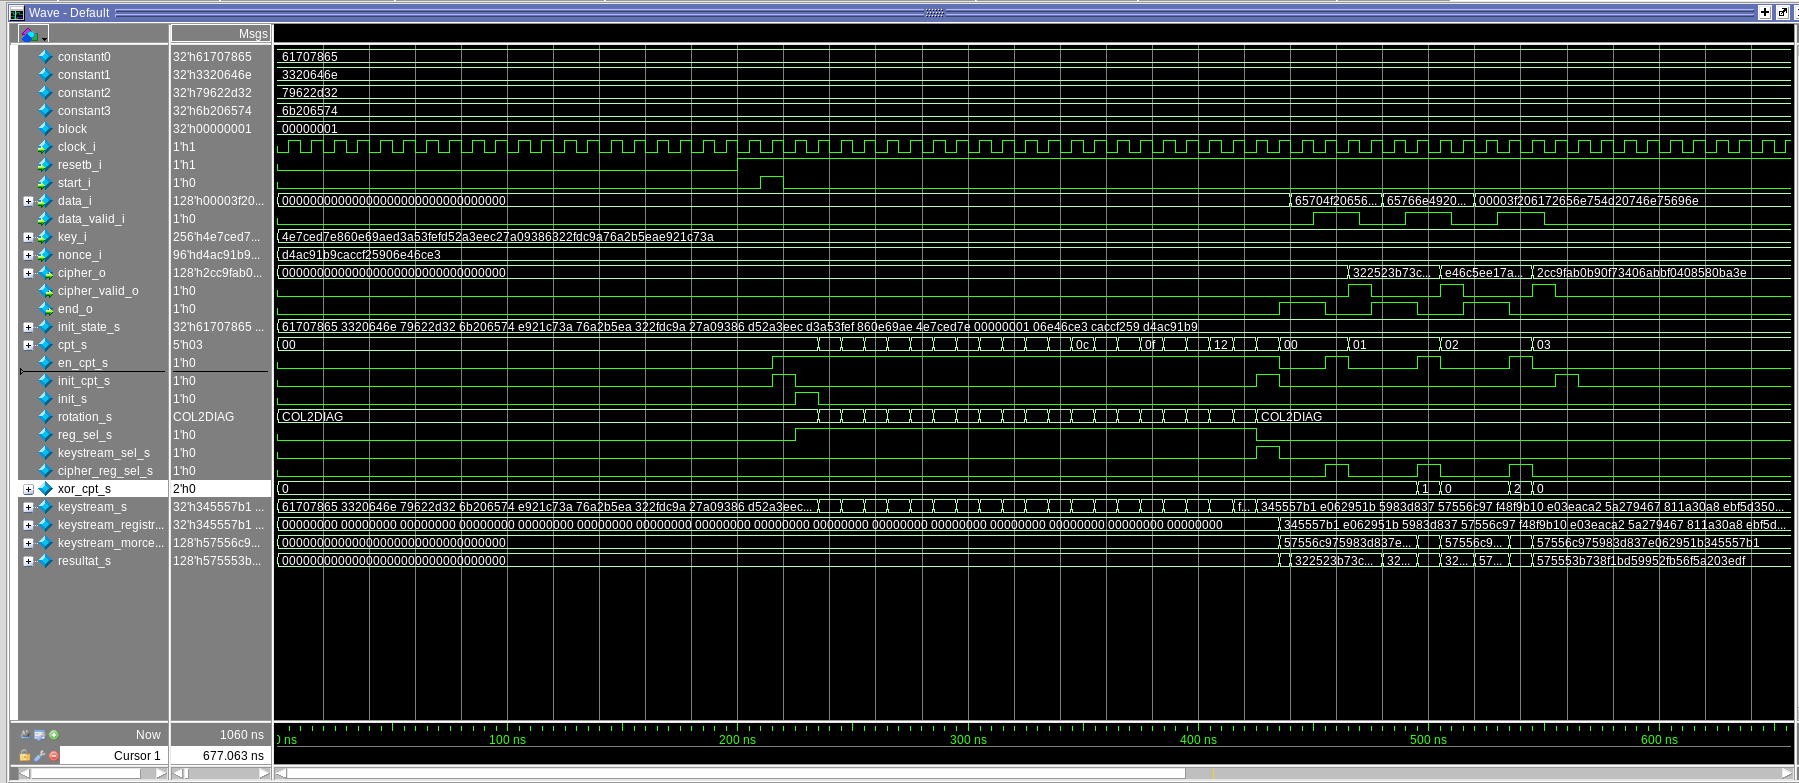
\includegraphics[width=1.2\linewidth]{testbenchtop.png}
    \caption{Simulation complète du module sous ModelSim.}
    \label{fig:placeholder_tb}
\end{figure}

On observe ainsi sur le chronogramme (\textit{waveform}) de ModelSim trois impulsions successives 
du signal \signal{cipher\_valid\_o}, ce qui indique la disponibilité et la bonne correspondance 
des messages chiffrés par rapport aux vecteurs de test attendus.

Le testbench vérifie ensuite par comparaison avec un XOR que les valeurs obtenues par mon algorithme \signal{cipher\_o}
correspondent aux vecteurs de chiffrements attendus par l'énoncé.

\begin{figure}
    \centering
    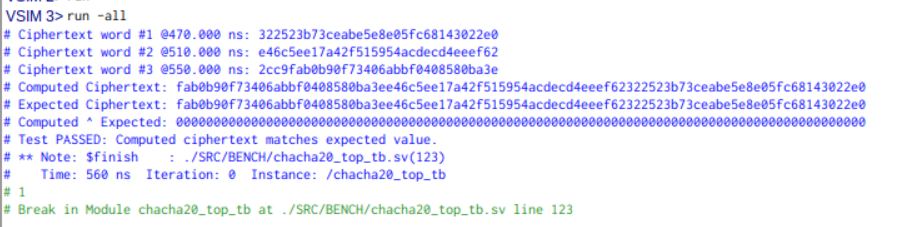
\includegraphics[width=1\linewidth]{tb.png}
    \caption{Validation de la simulation complète du module}
    \label{fig:placeholder}
\end{figure}

% ══════════════════════════════════════════════════════════════════════════════
\section{Problèmes rencontrés et solutions apportées}


\subsection{Difficultés rencontrées au cours du développement}


Durant le développement, j'ai initialement rencontré de nombreuses difficultés de compréhension du fonctionnement global de l'algorithme. De plus, j’ai aussi eu du mal à prendre en main le langage SystemVerilog. 


Avec l’aide de mon cours, j’ai pu réussir à terminer le projet à bien. 

En effet, une fois remis dans le bain avec mon cours en tête, j'ai été beaucoup à l’aise avec la création et le débogage des modules.




\subsection{Limites de l'implémentation et améliorations envisageables}

Il serait probablement possible de réduire l'état de ma machine d’état en regroupant plusieurs états au sein d’un même cycle d’horloge. Cependant, cela pourrait entraîner une diminution de la fréquence d’horloge maximale du circuit. 


\section{Conclusion}

De prime abord, j’ai trouvé ce projet très difficile, il ne s’est pour autant avéré simple.
Il m'aura permis de découvrir le SystemVerilog, qui, contrairement au C ou au Python, est un langage de description matérielle.


J’ai ressenti une difficulté croissante lors de l’avancement du projet. J’ai pu progresser à mon rythme et terminer le projet. Ce projet m’aura été très formateur sur la maîtrise du SystemVerilog.

De plus, j'ai grandement apprécié modéliser ce circuit, et contrairement à l'AES, Chacha20 ne possède pas de S-box, réduisant significativement le risque d'attaques matérielles telles que les attaques par canaux cachés. 




\end{document}
